\begin{enumerate}[label=\thesection.\arabic*.,ref=\thesection.\theenumi]
\numberwithin{equation}{enumi}

\item
Match the transfer functions of the second-order systems with the nature of the systems given below

\begin{tabular}{|c|c|}
\hline
Transfer function & Systems\\
 \hline
  P:$\frac{15}{{s^2+5s+15}}$  & 1:Overdamped \\
 Q:$\frac{25}{{s^2+10s+25}}$ & 2:Criticallydamped \\
 R:$\frac{35}{{s^2+18s+35}} &  3:Underdamped \\
 
\hline
\end{tabular}
\begin{align}
  (A)P-1,Q-2,R-3
\end{align}
\begin{align}
(B)P-2,Q-1,R-3
\end{align}
\begin{align}
 (C)P-3,Q-2,R-1
\end{align}
\begin{align}
 (D)P-3,Q-1,R-2
\end{align}
\solution The standard transfer function is H(s)=$\frac{\omega^2}{s^2+2\zeta\omega+\omega^2}\\
where \\"\omega"\ is \ natural \  frequency \\ and \ "\zeta" \ is\ damping\ factor\\

\newline then compare the given functions with this we get\\

 1. For Transfer function H(s)=$\frac{15}{s^2+5s+15}$, \\
\begin{align*}
     \omega^2 &= 15 \\ 2\zeta\omega &=5\\
    \text{then we get } \zeta &=$\sqrt{\frac{5}{12}} \textless 1
\end{align*}
2. For Transfer function H(s)=$\frac{25}{s^2+10s+25}$,\\
\begin{align*}
     \omega^2 &= 25 \\ 2\zeta\omega &=10\\
    \text{then we get } {\zeta} &= $\sqrt{\frac{5}{5}} = 1
\end{align*}
3. For Transfer function H(s)=$\frac{35}{s^2+18s+35}$,\\
\begin{align*}
    \omega^2 &= 35 \\ 2\zeta\omega &=18\\
    \text{then we get } {\zeta} &= $\sqrt{\frac{81}{35}} \textgreater 1
\end{align*}
The damping of a system can be described as being one of the following:
\newline \underline {Overdamped} &:
The system returns to equilibrium without oscillating.For this
\begin{align}
    \zeta \textgreater 1.
\end{align}
\newline \underline{Critically damped}&:
The system returns to equilibrium as quickly as possible without oscillating.
\newline For this 
\begin{align}
    \zeta = 1
\end{align}
\newline \underline{Underdamped}&:
The system oscillates(at reduced frequency compared to the undamped case) with the amplitude gradually decreasing to zero.
\newline For this 
\begin{align}
    0 \textless\zeta\textless1
\end{align}



\newline \underline{Undamped} &:
The system oscillates at its natural resonant frequency(\omega0).
\newline For this

\begin{align}
    \zeta = 0
\end{align}



\begin{tabular}{|c|c|}
\hline
 \multicolumn{2}{| c |}{Relation between damping and \zeta } \\
 \hline
 Types of Damping & \zeta(damping ratio)\\
 \hline
 Overdamped   & \zeta\textgreater 1 \\
 Criticallydamped & \zeta = 1 \\
 Underdamped &  0 \textless\zeta\textless1 \\
 Undamped    & \zeta = 0 \\
\hline
\end{tabular}
\newline \underline{Final Analysis}
\begin{itemize}
    \item As for P &: \zeta \textless 1
    \newline It\ is\ Underdamped\ system
    
    \item As for Q &: \zeta =1
     \newline It\ is\ critically\ damped\ system.
     
     \item As for R &: \zeta  \textgreater 1
    \newline It\ is\ an\ overdamped\ system.
  
  
   So,P-3,Q-2,R-1. Option (C) is correct.
\end{itemize}

\item Python code for the above damping graph :
\begin{lstlisting}
codes/ee18btech110012/damping.py
\end{lstlisting}

\item Python code for damped output taking unit step function as input:
\begin{lstlisting}
codes/ee18btech110012/unitstepdamping.py
\end{lstlisting}
1. For Transfer function H(s)=$\frac{15}{s^2+5s+15}$ \\
the damped output for step input is 
\begin{equation}
y(t)=25te^{-5t}u(t)
\end{equation}
2. For Transfer function H(s)=$\frac{25}{s^2+10s+25}$ \\
\begin{equation}
y(t)=\frac{30}{\sqrt{35}}e^{\frac{-5t}{2}}sin(\frac{\sqrt{35}}{2}t)u(t)
\end{equation}


3. For Transfer function H(s)=$\frac{35}{s^2+18s+35}$,\\
\begin{equation}
    y(t)=\frac{35}{2\sqrt{46}}(e^{(-9+\sqrt{46})t}-e^{(-9-\sqrt{46})t})u(t)
\end{equation}

%\usepackage{graphicx}
\begin{figure}
    \centering
    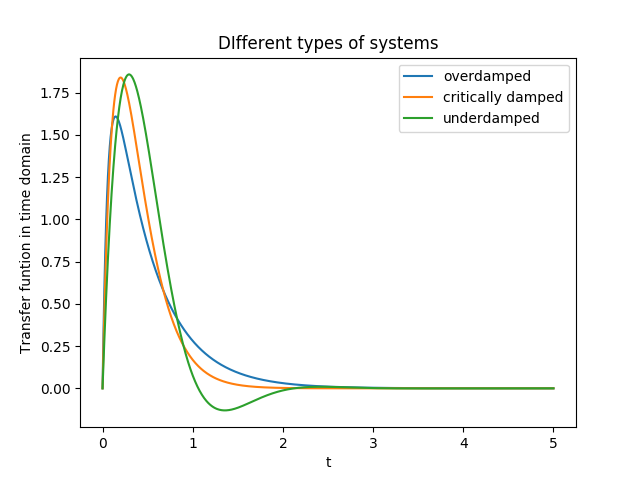
\includegraphics[width=0.7\linewidth]{Damping.png}
    \caption{Different systems based on \zeta}
    \label{fig:Graph}
\end{figure}

\begin{figure}
    \centering
    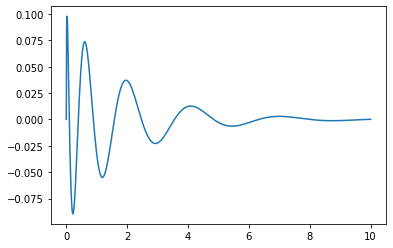
\includegraphics[width=0.7\linewidth]{unitstepdamping.png}
    \caption{Damped output for step input}
    \label{fig:Graph}
\end{figure}
\end{enumerate}
